\documentclass[12pt,letterpaper]{article}

\usepackage{assignments}
\usepackage{minted}

\begin{document}

\title{\vspace{-4ex}ECE521: Inference Algorithms and Machine Learning \\
University of Toronto\\ \  \\
Assignment 2: \\Logistic Regression and Neural Networks}
\date{\vspace{-8ex}TA: Use Piazza for Q\&A \\ Due date: Feb 27 11:59 pm, 2017 \\ Electronic submission to: \href{mailto:ece521ta@gmail.com}{ece521ta@gmail.com} }

\maketitle

\section*{General Note:}
\begin{itemize}
\item The purpose of this assignment is to investigate the classification performance of logistic regression and neural networks. In this assignment, you will gain some experience in training a neural network and will use an effective way to avoid overfitting. All the implementations need to be done using Python and TensorFlow. You are encouraged to look up TensorFlow APIs for useful utility functions,  at: \url{https://www.tensorflow.org/api_docs/python/}.
\item Full points are given for complete solutions, including justifying the choices or assumptions you made to solve each question. Both a written report and your complete source code (as an appendix and separate files) should be included in the final submission.
\item Homework assignments are to be solved by yourself or in groups of two. You are encouraged to discuss the assignment with other students, but you must solve it within your own group. Make sure to be closely involved in all aspects of the assignment. If you work in a group, please indicate the contribution percentage from each group member at the beginning of your report.
\end{itemize}


\section*{notMNIST Dataset}

The dataset that we will use in this assignment is a permuted version of notMNIST\footnote{\url{http://yaroslavvb.blogspot.ca/2011/09/notmnist-dataset.html}}, which contains 28-by-28 images of 10 letters (A to J) in  different fonts. This dataset has 18720 instances, which can be divided into different sets for training, validation and testing. The provided file is in \textbf{.npz} format which is for Python. You can load this file as follows.

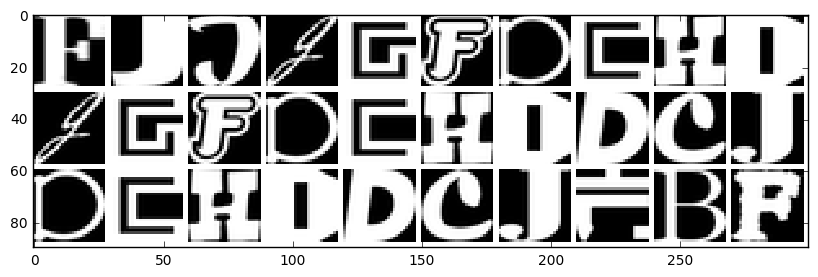
\includegraphics[scale=0.6]{multiclass.png}

\begin{minted}{python}
with np.load("notMNIST.npz") as data:
    Data, Target = data ["images"], data["labels"]
    np.random.seed(521)
    randIndx = np.arange(len(Data))
    np.random.shuffle(randIndx)
    Data = Data[randIndx]/255.
    Target = Target[randIndx]
    trainData, trainTarget = Data[:15000], Target[:15000]
    validData, validTarget = Data[15000:16000], Target[15000:16000]
    testData, testTarget = Data[16000:], Target[16000:]
\end{minted}

\subsection*{Two-class notMNIST dataset}
We use the following script to generate a smaller dataset that only contains the images from two letter classes: ``C''(the positive class) and ``J''(the negative class). This smaller subset of the data contains 3500 training images, 100 validation images and 145 test images.

%\begin{figure*}
%\centering
%\vspace{-0.1in}
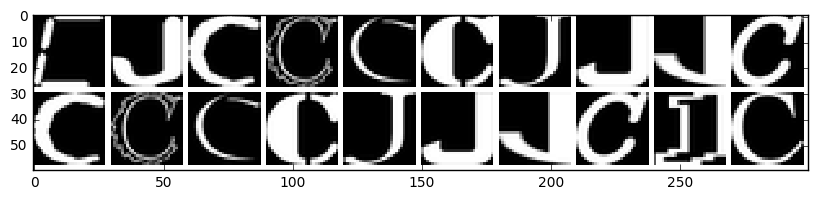
\includegraphics[scale=0.6]{binary.png}
%\vspace{-0.1in}
%\end{figure*}

\begin{minted}{python}
with np.load("notMNIST.npz") as data :
    Data, Target = data ["images"], data["labels"]
    posClass = 2
    negClass = 9
    dataIndx = (Target==posClass) + (Target==negClass)
    Data = Data[dataIndx]/255.
    Target = Target[dataIndx].reshape(-1, 1)
    Target[Target==posClass] = 1
    Target[Target==negClass] = 0
    np.random.seed(521)
    randIndx = np.arange(len(Data))
    np.random.shuffle(randIndx)
    Data, Target = Data[randIndx], Target[randIndx]
    trainData, trainTarget = Data[:3500], Target[:3500]
    validData, validTarget = Data[3500:3600], Target[3500:3600]
    testData, testTarget = Data[3600:], Target[3600:]
\end{minted}


\section{Logistic Regression [18 pt]}

\subsection{Binary cross-entropy loss [10 pt.]}

The MSE loss function works well for typical regression tasks in which the model outputs are real values. Despite its simplicity, MSE can be overly sensitive to mislabelled training examples and to outliers. A more suitable loss function for the classification task is the cross-entropy loss, which compares the log-odds of the data belonging to either of the classes. Because we only care about the probability of a data point belonging to one class, the real-valued linear prediction is first fed into a sigmoid function $\sigma(z) = \frac{1}{1+e^{-z}}$ that ``squashes'' the real-valued output to fall between zero and one. The model output is therefore $\hat{y}(\mathbf{x}) = \sigma(W^T\mathbf{x} + b)$. The cross-entropy loss is defined as:
\begin{align*}
  \mathcal{L} =& \mathcal{L}_{\mathcal{D}} + \mathcal{L}_W \\ =& \sum_{m=1}^M \frac{1}{M} \bigg[-{y}^{(m)}\log\hat{y}(\mathbf{x}^{(m)}) - (1-{y}^{(m)})\log(1-\hat{y}(\mathbf{x}^{(m)}))\bigg]
   + \frac{\lambda}{2} \|W\|^2_2
\end{align*}
The sigmoid function is often called the logistic function and hence a linear model with the cross-entropy loss is named ``logistic regression''. 

\begin{enumerate}
  \item \textbf{Learning}: Write a TensorFlow script that implements logistic regression and the cross-entropy loss (and you want to use the \textit{tf.nn.sigmoid\_cross\_entropy\_with\_logits} utility function to avoid numerical underflow). Set the weight-decay coefficient $\lambda = 0.01$. Train the logistic regression model using SGD and a mini-batch size $B=500$ on the \textit{two-class notMNIST} dataset. Plot the best training and testing curves for both cross-entropy loss and classification accuracy vs. the number of updates after tuning the learning rate. Report the best test classification accuracy obtained from the logistic regression model.  [2 pt.]
{\color{red}
  \textbf{Answers:}
  One possible implementation
}
\begin{minted}{python}
def buildGraph_logistic():
    # Variable creation
    W = tf.Variable(tf.truncated_normal(shape=[64,1], stddev=0.5), name='weights')
    b = tf.Variable(0.0, name='biases')
    X = tf.placeholder(tf.float32, [None, 64], name='input_x')
    y_target = tf.placeholder(tf.float32, [None,1], name='target_y')
    wd_lambda = tf.placeholder("float32", name='wd_lambda')


    # Graph definition
    y_logit = tf.matmul(X,W) + b
    y_predicted = tf.nn.sigmoid(y_logit)

    # Error definition
    crossEntropyError = tf.reduce_mean(
                    tf.nn.sigmoid_cross_entropy_with_logits(y_logit, y_target), 
                                  name='mean_cross_entropy')
    weight_loss = tf.reduce_sum(W*W) * wd_lambda * 0.5

    loss = crossEntropyError + weight_loss
    # Training mechanism
    optimizer = tf.train.GradientDescentOptimizer(learning_rate = 0.01)
    #optimizer = tf.train.AdamOptimizer(learning_rate = 0.001)
    train = optimizer.minimize(loss=loss)
    return W, b, X, y_target, y_predicted, crossEntropyError, wd_lambda, train
\end{minted}




  \item \textbf{Beyond plain SGD}: With the same weight-decay coefficient $\lambda = 0.01$ and mini-batch size $B=500$, train the logistic regression model with the Adam optimizer\footnote{\url{https://arxiv.org/abs/1412.6980}} (use the \textit{tf.train.AdamOptimizer} function). Plot the best training and testing curves for both the cross-entropy loss and the classification accuracy after tuning the learning rate. Compare the two sets of learning plots: those from SGD and those from using the Adam-Optimizer curve. Comment on their differences, and explain how the Adam optimizer may help learning from the notMNIST dataset. (\textbf{For the rest of the assignment, you should use the Adam optimizer in all numerical experiments.}) [2 pt.]
  
  \item \textbf{Comparison with linear regression}: Set the weight decay coefficient to zero. Write a TensorFlow script to find the optimal linear regression weights on the \textit{two-class notMNIST} dataset using the ``normal equation'' of the least squares formula. Compare the train, validation and test classification of the least squares solution to the optimal logistic regression learnt without weight decay. What do you observe about the effect of the cross-entropy loss on the classification performance?  To help explain your observation, you may wish to plot the cross-entropy loss vs squared-error loss as a function of the prediction $\hat{y}$ within the interval [0, 1] and a dummy target $y=0$ in 1-D. [2 pt.] 

\item \textbf{Maximum likelihood estimation}: In lecture we derived, from an i.i.d. data set, the MLE parameters of a Gaussian whose mean is parameterized by a linear function using weights $W$ and $b$. It turned out that the MLE method was equivalent to minimizing the squared $\ell_2$ loss from linear regression. Similarly, the cross-entropy loss can be derived from the MLE principle by assuming a Bernoulli distribution for the likelihood of the training labels $y \in \{0,1\}$, i.e. $P(y=1|\mathbf{x}, W) = 1 - P(y=0|\mathbf{x}, W) = \hat{y}(\mathbf{x})$. We can write the Bernoulli distribution parameterized by $W$ more concisely as $P(y | \mathbf{x}, W) = \hat{y}(\mathbf{x})^y(1-\hat{y}(\mathbf{x}))^{(1-y)}$. Show that minimizing the cross-entropy loss is equivalent to maximizing the log-likelihood of the training data under the Bernoulli assumption.  [4 pt.]

{\color{red} 
\textbf{Answer: }
Under Bernoulli assumption, the log likelihood of a single data point can be written as:
\begin{align*}
  \log P(y | \mathbf{x}, W) = y\log\hat{y}(\mathbf{x}) + (1-y) \log(1-\hat{y}(\mathbf{x}))
\end{align*}
Maximum likelihood estimator is obtained by summing over all the data points:
\begin{align*}
  \max_W \sum_m \log P(y^{(m)} | \mathbf{x}^{(m)}, W) = \sum_m [ y^{(m)}\log\hat{y}(\mathbf{x}^{(m)}) + (1-y^{(m)}) \log(1-\hat{y}(\mathbf{x}^{(m)}))]
\end{align*}
Hence, maximizing the Bernoulli likelihood is equivalent to minimizing the cross-entropy loss.
}
\end{enumerate}

\subsection{Multi-class classification [8 pt.]}

\begin{enumerate}
\item Suppose a classifier operates by assigning each input, $\mathbf{x}$, to
the class with the largest \textit{a posteriori} probability. Show that this
classifier represents a minimum-loss system if the penalty for
misclassification is equal for each class. [3 pts]

{\color{red} 
\textbf{Answer: }
Consider regions $R_k$ for $k \in \{1, \dots, C\}$ over $C$ classes.
\begin{align*}
  p(\text{correct class}) &= \sum_{k=1}^C p(\mathbf{x}\in R_k, C_k) \\
                          &=\sum_{k=1}^C p(\mathbf{x}\in R_k|C_k) p(C_k) \\
  &=\sum_{k=1}^C \int_{R_k}p(\mathbf{x}\in R_k|C_k) p(C_k)
\end{align*}
To maximize this, we maximize $p(\mathbf{x}|C_k)p(C_k)$ for all $\mathbf{x}$. Because $p(\mathbf{x})$ is constant over all classes, maximizing $p(\mathbf{x}|C_k)p(C_k)$ is equivalent to maximizing
\begin{align*}
  p(C_k|\mathbf{x}) =  \frac{p(\mathbf{x}\in R_k|C_k) p(C_k)}{p(\mathbf{x})}
\end{align*}
Therefore, we choose the class with the maximum posterior probability.
}

\item Consider a more complex loss matrix, $\mathbf{L}$, in which $L_{jk}$
represents the penalty for misclassification to class $j$ when the pattern in
fact belongs to class $k$. Under what condition should classification of
$\mathbf{x}$ to class $C_j$ be made if the total loss is to be minimized? [3
pts]

{\color{red} 
\textbf{Answer: }
The loss associated with points really in class k is:
\begin{gather*}
  \text{loss}_k = \sum_{j=1}^C L_{kj}\int_{R_j}p(\mathbf{x}|C_k) d\mathbf{x}
\end{gather*}
The total loss is given by
\begin{gather*}
  \sum_{k=1}^C \text{loss}_k = \sum_{j=1}^C\int_{R_j} \left\{ \sum_{k=1}^C  L_{kj}p(\mathbf{x}|C_k)\right\} d\mathbf{x}
\end{gather*}
Minimizing the integrand at each $\mathbf{x}$ gives classification to class $C_j$ iff
\begin{gather*}
  \sum_{k=1}^C  L_{kj}p(\mathbf{x}|C_k)p(C_k) < \sum_{k=1}^C  L_{ki}p(\mathbf{x}|C_k)p(C_k), \quad \forall i\ne j
\end{gather*}
As $p(\mathbf{x})$ is constant across classes, this is equivalent to
\begin{gather*}
  \sum_{k=1}^C  L_{kj}p(\mathbf{x}|C_k) < \sum_{k=1}^C  L_{ki}p(\mathbf{x}|C_k), \quad \forall i\ne j
\end{gather*}
}

\item  Write a TensorFlow script that implements logistic regression using softmax output and with multi-class cross-entropy loss (you will want to use the \textit{tf.nn.softmax\_cross\_entropy\_with\_logits} utility function, to avoid numerical underflow). Regularize the weights with $\lambda = 0.01$. Using a mini-batch size of $B=500$ and a learning rate that you tune, train the logistic regression model on the full \textit{notMNIST} dataset with 10 classes. For the best value of learning rate, plot the training and testing curves for both cross-entropy loss and classification accuracy vs.\ the number of updates. Report the best test classification accuracy obtained from the logistic regression model. Is the training and testing classification performance better or worse than the binary-class problem in question 1.1? Explain intuitively the difference. [2 pts]

{\color{red}
  \textbf{Answers:}
  One possible implementation
}
\begin{minted}{python}
def buildGraph_softmax():
    # Variable creation
    W = tf.Variable(tf.truncated_normal(shape=[784,10], stddev=0.5), 
                    name='weights')
    b = tf.Variable(tf.zeros([10,]), name='biases')
    X = tf.placeholder(tf.float32, [None, 28, 28], name='input_x')
    y_target = tf.placeholder(tf.float32, [None,], name='target_y')
    
    wd_lambda = tf.placeholder("float32", name='wd_lambda')


    # Graph definition
    y_onehot = tf.to_float(tf.equal(tf.expand_dims(y_target, 1),
                                    tf.to_float(tf.constant(
                                        np.arange(10).reshape(1,-1)))))
    X_flatten = tf.reshape(X, [-1, 28*28])
    y_logit = tf.matmul(X_flatten,W) + b
    y_predicted = tf.nn.softmax(y_logit)

    # Error definition
    crossEntropyError = tf.reduce_mean(
                        tf.nn.softmax_cross_entropy_with_logits(y_logit, y_onehot), 
                                  name='mean_cross_entropy')
    weight_loss = tf.reduce_sum(W*W) * wd_lambda * 0.001

    loss = crossEntropyError + weight_loss
    # Training mechanism
    optimizer = tf.train.AdamOptimizer(learning_rate = 0.001)
    train = optimizer.minimize(loss=loss)
    return W, b, X, y_target, y_predicted, crossEntropyError, wd_lambda, train
\end{minted}



\end{enumerate}

\section{Neural Networks [28 pt.]}

In this part, we use a neural network to classify the letters in the dataset. In all of the tasks, use ReLU activation functions, a cross-entropy cost function, and a softmax output layer. As an estimate of the running time, training the following neural networks will not take more than an hour on an Intel core i7 1.73-GHz CPU with 4 GB of RAM. Because you will be running a few experiments, it is a good idea to save (``checkpoint'') your model during training at 25\%, 50\%, 75\% and 100\% of the training process, to four separate models. The function \textit{tf.saver} can come in handy for checkpointing and you may reload your model later for inspection or use.


\subsection{Geometry of neural networks [6 pt.]}
\begin{enumerate}
\item Consider learning a single sigmoid neuron to classify a \textit{linearly separable} binary classification dataset (i.e. a hyperplane decision boundary can perfectly separate out the positive and the negative examples). Show that \textit{without} weight decay, the length of optimal weights vector $W$ learnt on this dataset will be unbounded. In other words, show that the L2 norm of the optimal weights $\|W^* \|_2 = \infty$.  [2 pt.]

  {\color{red} 
\textbf{Answer: }
A sigmoid neuron computes a logistic transformation of the weighted sum of its inputs:
\begin{align*}
  \hat{y}(\mathbf{x}) = \sigma({W^*}^T\mathbf{x})
\end{align*}
We will use cross-entropy loss for training such sigmoid neuron with the optimal weight vector  $W^*$, i.e.:
\begin{align*}
  W^* = \arg\min_W \quad \sum_m [- y^{(m)}\log\hat{y}(\mathbf{x}^{(m)}) - (1-y^{(m)}) \log(1-\hat{y}(\mathbf{x}^{(m)}))]
\end{align*}
Under a linearly separable dataset, the cross-entropy loss will be zero for the optimal weight vector $W^*$, i.e. it predicts all the training examples perfectly. And the gradient w.r.t. to the weights is also zero for the optimal weights:
\begin{align*}
  \sum_m (\hat{y}(\mathbf{x}^{(m)}) - y^{(m)})\mathbf{x} = 0.
\end{align*}
The labels $y^{(m)}$ are ones and zeros. Assume all the input feature $\mathbf{x}$ are non-zero and bounded, the model prediction $\hat{y}$ has to be either exact zero or one to achieve zero gradient. Let a training case $\mathbf{x}^{(i)}$ have a positive label, ie $y^{(i)}= 1$, then the optimal weight vector $W^*$ will satisfy the prediction $\hat{y}$ to be one:  
\begin{align*}
  {W^*}^T\mathbf{x}^{(i)} = \infty \quad \Rightarrow \quad \hat{y}(\mathbf{x}^{(i)}) = \sigma({W^*}^T\mathbf{x}^{(i)}) = 1 = y^{(i)}\\
\end{align*}
Similarly for a negative training case $\mathbf{x}^{(j)}$ and $y^{(j)}= 0$, then the optimal weight vector $W^*$ will be:
\begin{align*}
  {W^*}^T\mathbf{x}^{(j)} = -\infty \quad \Rightarrow \quad \hat{y}(\mathbf{x}^{(j)}) = \sigma({W^*}^T\mathbf{x}^{(j)}) = 0 = y^{(j)}
\end{align*}
Hence, the $\ell_2$ norm of the optimal weight vector $\sqrt{{W^*}^T{W^*}} = \infty$. 
}

\item Consider learning a single sigmoid neuron on a linearly \textit{inseparable} binary classification problem. Show that \textit{without} weight decay, the length of optimal weights vector $W$ learnt on this dataset will always be bounded. In other words, show that the L2 norm of the optimal weights $\|W^* \|_2 < \infty$. [2 pt.]

{\color{red} 
\textbf{Answer: }
Use the same setup as the question above, let us consider the cross-entropy loss function:
\begin{align*}
  \min_W \quad \sum_m [- y^{(m)}\log\hat{y}(\mathbf{x}^{(m)}) - (1-y^{(m)}) \log(1-\hat{y}(\mathbf{x}^{(m)}))]
\end{align*}
Because this is a linearly inseparable dataset, there will be some training examples get mislabeled by the sigmoid neuron (logistic regression). Consider a mislabeled training example $\mathbf{x}^{(i)}$ that is in the positive class, ie $y^{(i)}= 1$. Assume the norm of the optimal weights are unbounded:
\begin{align*}
  {W^*}^T\mathbf{x}^{(i)} = -\infty \quad \Rightarrow \quad \hat{y}(\mathbf{x}^{(i)}) = \sigma({W^*}^T\mathbf{x}^{(i)}) = 0 \quad \Rightarrow \quad - y^{(i)}\log\hat{y}(\mathbf{x}^{(i)}) = \infty\\
\end{align*}
Then the cross-entropy would be infinite under the unbounded optimal weights. Therefore, the $\ell_2$ norm of the optimal weights that minimize the cross-entropy has to be bounded, i.e. $\sqrt{{W^*}^T{W^*}} = \infty$ 
}

\item Consider learning a single hidden layer neural network to classify a linearly \textit{inseparable} binary classification dataset \st{(i.e. a hyperplane decision boundary can perfectly separate out the positive and the negative examples)}. For all the weight matrices in the neural network, we can first flatten each weight matrix into a vector and let $\text{vec}\{W\}$ denote the vector that is the concatenation of all the flattened weight matrices. Under cross-entropy loss \textit{without} weight decay, give constructive examples to show that some locally optimal solutions have bounded weight vector $\|\text{vec}\{W^*\}\|_2<\infty$ and that some other locally optimal solutions have unbounded weight vector $\|\text{vec}\{W^*\}\|_2 = \infty$.  [2 pt.]

{\color{red} 
\textbf{Answer: }
$\|\text{vec}\{W^*\}\| = \infty$ case:
Consider a neural network that has the same number of hidden units as the training example, and assume the first hidden layer learns to map each training point to a specific neuron and each neuron only activates for a particular training example so there is one-to-one correspondence between the neuron and training example. Then such neural network can effectively map the training examples into a hidden space that is linearly separable space. We already know from the previous question that under the linearly separable condition, the norm of the weights is unbounded. 

$\|\text{vec}\{W^*\}\| < \infty$ case:
Consider a neural network that all the hidden units in the hidden layer has the identical incoming weights. Furthermore, all the incoming weights of the output neuron are also identical. Any gradient descent algorithm will not break the weight symmetry under such degenerated neural network. Hence such neural network will only have two degrees of freedom by changing the scalar value of the first hidden layer weights and the scale value of the output weights. This is just a degenerated case of a sigmoid neuron classifying linearly inseparable dataset. Therefore, the norm of the optimal weights is bounded under such construction.
}

\end{enumerate}

\subsection{Feedforward fully connected neural networks [8 pt.]}
\label{subsec:fcnn}
Implement a simple neural network with one hidden layer and 1000 hidden units. Train your neural network on the entire notMNIST training set of ten classes. Because the neural network loss functions are non-convex, a proper weights initialization scheme is crucial to prevent vanishing gradient during back-propagation as a result of learning stuck at a plateau at the beginning of the training. You will use the Xavier initialization to initialize the weight matrices for all the neural networks in this assignment. That is, each weight matrix is initialized from zero-mean independent Gaussians whose variance is $3 / (\#input\_units + \#output\_units )$. Unlike the weight matrices, the bias units will be initialized to zero.




\begin{enumerate}
  \item  \textbf{layer-wise building block:} Write a \underline{vectorized} Tensorflow Python function that takes the hidden activations from the previous layer then return \textit{the weighted sum of the inputs}(i.e. the $\mathbf{z}$) for the current hidden layer. You will also initialize the weight matrix and the biases in the same function. You should use Xavier initialization for the weight matrix. Your function should be able to compute the weighted sum for all the data points in your mini-batch at once using matrix matrix multiplication. It should not contain loops over the training examples in the mini-batch. The function should accept two arguments, the input tensor and the number of the hidden units. Include the snippets of the Python code. [2 pt.]

{\color{red}
  \textbf{Answers:}
  One possible implementation
}
\begin{minted}{python}
def linear(x, numHidden):
    numInput = int(x.get_shape()[1])
    tmp = (numInput+numHidden)
    weights = tf.Variable(tf.random_normal([numInput, numHidden], 
                          stddev=tf.sqrt(1./tmp)), 
                          name = "w")
    bias = tf.Variable(tf.zeros( [numHidden,]), name="b")
    weights_loss = tf.reduce_sum(weights**2)/2.
    tf.add_to_collection("weights_loss", weights_loss)
    return tf.nn.bias_add(tf.matmul(x, weights), bias)
\end{minted}
  \item  \textbf{Learning:} Use your function from the previous question to build your neural network model with ReLU activation functions in TensorFlow and \textit{tf.nn.relu} can be useful. For training your network, you are supposed to find a reasonable value for your learning rate. You should train your neural network for different values of learning rate and choose the one that gives you the fastest convergence in terms of the training loss function. (You might want to ``babysit'' your experiments and terminate a particular run prematurely as soon as you find out that the learning rate value is not very good.) Trying 3 different values should be enough. You may also find it useful to apply a small amount of weight decay to prevent overfitting. (e.g. $\lambda = 3e-4$.) On the training set, validation set and test set, record your classification errors and cross-entropy losses after each epoch. Plot the training, validation, and test classification error vs. the number of epochs. Make a second plot for the cross-entropy loss vs. the number of epochs. Comment on your observations. [4 pt.]

{\color{red}
  \textbf{Answers:}
  One possible implementation
}
\begin{minted}{python}
x = tf.placeholder(tf.float32, shape=(None, 28,28))
y_target = tf.placeholder(tf.float32, [None,], name='target_y')
y_onehot = tf.to_float(tf.equal(tf.expand_dims(y_target, 1),
                                tf.to_float(tf.constant(
                                    np.arange(10).reshape(1,-1)))))
x_reshape = tf.reshape(x, [-1, 28*28])
h = x_reshape
for i in range(1):
    h = tf.nn.relu(linear(h, 1000))
yhat = (linear(h, 10))
crossEntropyError = tf.reduce_mean(
                tf.nn.softmax_cross_entropy_with_logits(yhat, y_onehot))
weightsError = tf.add_n(tf.get_collection("weights_loss"))
loss = crossEntropyError + 3e-4*weightsError
acc = tf.reduce_mean(tf.to_float(
                    tf.equal(tf.to_float(tf.arg_max(yhat, 1)), 
                             tf.to_float(y_target))))
train_op = tf.train.AdamOptimizer(learning_rate=0.001,).minimize(loss)
\end{minted}


  \item \textbf{Early stopping:} \textit{Early stopping} is the simplest procedure to avoid overfitting. Determine and highlight the early stopping point on the classification error plot from \st{question 1} {\color{red} question 2.2.2}, and report the training, validation and test classification error at the early stopping point. Are the early stopping points the same on the two plots? Why or why not? Which plot should be used for early stopping, and why? [2 pt.]
\end{enumerate}

\subsection{Effect of hyperparameters [4 pt.]}
\begin{enumerate}
   \item  \textbf{Number of hidden units:}
Instead of using 1000 hidden units, train different neural networks with $[100, 500, 1000]$ hidden units. Find the best validation error for each one. Choose the model which gives you the best result, and then use it for classifying the test set. What is the number of test errors {\color{red}(or test classification errors)}? In one sentence, summarize your observation about the effect of the number of hidden units on the final results. [2 pt.]

   \item  \textbf{Number of layers:}
     For this task, train a neural network with two hidden layers of 500 hidden units each (1000 total). Plot the number of training and validation errors {\color{red}(or training and validation classification errors)} vs. the number of epochs. What is the final validation error when training is complete? Using the test set, compare this architecture with the one-layer case. [2 pt.]
\end{enumerate}

\subsection{Regularization and visualization [6 pt.]}
Dropout is a powerful technique to reduce overfitting and to enhance the overall performance of the neural network. Using the same architecture in Sec.~\ref{subsec:fcnn}. 
\begin{enumerate}
\item  \textbf{Dropout}: Introduce dropout on the hidden layer of the neural network (with dropout rate 0.5) and train you neural network. As you know, dropout should only be used in the training procedure, and the ``mean network'' should be used instead during the evaluation. Plot the number of training and validation errors {\color{red}(or training and validation classification errors)} vs the number of epochs. compare the results with the case that we do not have any dropout. Summarize the observed effect of dropout. (You may want to use the \textit{tf.nn.dropout} utility function.) [2 pt.]
\item  \textbf{Visualization}: It is generally hard to figure out what the hidden neurons are doing in a neural network. However, one can visualize the incoming weight vector to each hidden neuron in the first hidden layer as an image and inspect what that neuron has learnt from the dataset. For the neural networks we have trained in this assignment, we can visualize the values of the 28x28 incoming weights of each hidden units in the first layer as a grey-scale image. For the models trained with and without dropout, checkpoint the model during training at 25\%, 50\%, 75\% and 100\% of the early stopping point. For each of the checkpoints, make a figure visualizing the 1000 neurons in the first hidden layer. Comment on the learning progression of the hidden neurons, and comment on any difference between the dropout model and the one without dropout. [4 pt.]
\
\end{enumerate}

\subsection{Exhaustive search for the best set of hyperparameters  [4 pt.]}
As you have seen in the previous tasks, hyperparameters play a very important role in neural networks. So, finding the best set of hyperparameters is a critical step toward getting a good result. The most reliable way is exhaustive search, which is trying many different sets of values and picking the model with the lowest validation error. However, this procedure is computationally expensive and it needs to be done with a GPU\footnote{\url{http://www.nvidia.ca/object/what-is-gpu-computing.html}}. A GPU divides a large task into many smaller ones and assigns them to different cores for parallel processing. Unfortunately, not all of you may have access to a GPU, but fortunately we can still use the idea of parallel processing. The whole class can be a GPU or a cluster server, and each student group will be one of its computation nodes!
To achieve this goal, each group will perform some experiments and report their results.
We will compare all the results and let you know the best model and the best test error rate that can be achieved.
\begin{enumerate}
  \item \textbf{Random search}: First, try to set the random seeds in Numpy and TensorFlow libraries differently from other groups. (e.g. seed using the time of your experiments or some combination of your student IDs). Randomly sample the \textit{natural log of learning rate} uniformly between -7.5 and -4.5, the \textit{number of layers} from 1 to 5, the \textit{number of hidden units per layer} between 100 and 500, and the natural log of weight decay coefficient uniformly from the interval $[-9, -6]$. Also, randomly choose your model to use \textit{dropout} or not. Using these hyperparameters, train your neural network and report its validation and test \textit{classification error}. Repeat this task for five models, and report their results. [2 pt.] 
    
  \item \textbf{Exchange ideas among the groups }: Collaboration is the key ingredient of major scientific progress and innovation. Advances in the fields of artificial intelligence and machine learning tend to depend on the rapid sharing of ideas and datasets. You will now exchange and compare your experimental results and the hyperparameter settings with other groups. (Yes, this means you will have to talk to other students in the class in person or use Piazza). You will now use the best hyperparameter you heard from someone who heard from someone else and report the best test error rate that can be achieved under the hyperparameter space in this question. Let us hope the wisdom the crowd will converge to a single best model. [2 pt.]
\end{enumerate}




\end{document}

